\documentclass{jarticle}
\usepackage[dvipdfmx]{graphicx}
\usepackage{listings,jlisting,url,here}

\lstset{%
  language={C},
  basicstyle={\small},%
  identifierstyle={\small},%
  commentstyle={\small\itshape},%
  keywordstyle={\small\bfseries},%
  ndkeywordstyle={\small},%
  stringstyle={\small\ttfamily},
  frame={tb},
  breaklines=true,
  columns=[l]{fullflexible},%
  numbers=left,%
  xrightmargin=0zw,%
  xleftmargin=3zw,%
  numberstyle={\scriptsize},% stepnumber=1,
  numbersep=1zw,%
  lineskip=-0.5ex%
}
% xなんちゃらが変数,進捗書く
\newcommand{\xb}{催涙スプレーのゲージを表示}

% []内の数が引数,#数字で引数読む
\newcommand{\pitem}[1]{
  \item #1
}

\title{最終グループレポート}
\author{6119019207 矢野大暉}
\date{\number\year/\number\month/\number\day 提出}

\begin{document}
\maketitle

\section{ゲーム内容、操作方法(マニュアル)}
%\subsection{ゲームのタイトル}
%AGENT 3
%
%\subsection{ジャンル}
%脱出ゲーム
%
%\subsection{概略}
%ゲームの設定は,「犯罪組織に盗まれた金塊を組織に潜入して,複数のプレイヤーと協力して,組織的に取り返>す」といった設定である.
%本ゲームは,同一のサーバに接続した複数のプレイヤーが協力する脱出ゲームである.プレイヤーは出入り口か>らスタートし,敵キャラ(敵),監視カメラに見つからないように,ステージ上に設置された金塊をゲットし再び>敵,監視カメラに見つからないように出入り口に帰ってくるゲームである.
%ステージは複数用意されており,ステージが上がるごとに敵や監視カメラを増やすことで難易度を向上させる.
%
%プレイヤーは敵キャラや監視カメラに対して妨害を行うことで,他プレイヤーが金塊を取るためのアシストを行>うことができる.
%プレイヤーが行うことができる妨害として以下が挙げられる.
%\begin{itemize}
%\item 敵キャラに話しかける → 敵の視界の固定
%\item 監視カメラのハッキング → 監視カメラが一時的に停止
%\item 敵キャラに催涙スプレー → 敵の視界が無効化
%\end{itemize}
%
%\subsection{プレイ人数}
%3人
%
%\subsection{操作方法}
%本ゲームはジョイパッドでの操作を行う.
%
%移動 : ジョイパッドのアナログスティック\\
%ハッキング : 1ボタン\\
%催涙スプレー : 2ボタン\\
%会話 : 3ボタン\\
%金塊を取得 : 4ボタン\\
%;;
%
%\subsection{画面構成}
%ゲームのイメージ図を図\ref{fig:gameimg}に示す.
%
%\begin{figure}[H]
%\begin{center}
%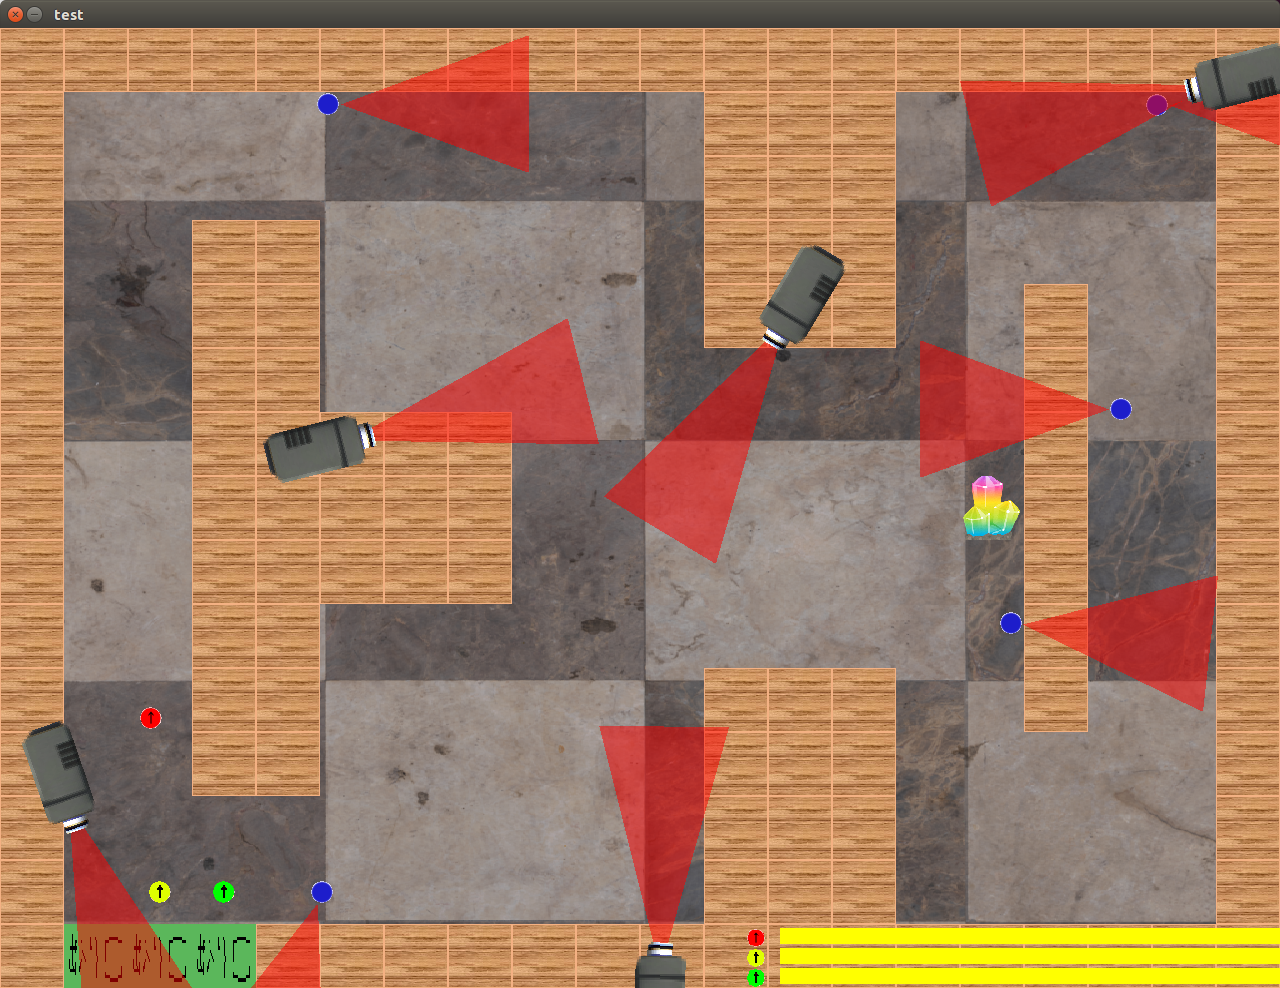
\includegraphics[width=\linewidth]{./zu/stage1.png}
%\caption{ゲームウィンドウ}
%\label{fig:gameimg}
%\end{center}
%\end{figure}
%
%赤、黄、緑で示しているのがプレイヤー,青で示しているのが敵(NPC)である.
%赤の三角形がそれぞれ敵、監視カメラの視界であり、プレイヤーが金塊を持った時にこの中に入るとゲームオーバーになる。
%敵キャラ,監視カメラの扇形の物体は視界を表しており,この中にプレイヤーがいるとプレイヤーが「見つかっ>た」判定となる.
%
%\subsection{勝敗,クリア,終了条件}
%クリア条件は,プレイヤーが金塊を取って出入り口へ向かうことができればゲームクリアである.
%ゲームオーバー条件はプレイヤーが敵キャラまたは監視カメラに見つかってしまうことである.
%
%\subsection{その他の特徴}
%敵キャラの動きはルールベース型AIを採用している.進捗状況によっては,強化学習なども用いる.
%敵キャラのAIの具体例としては以下が挙げられる.
%\begin{itemize}
%\item 敵がプレイヤーに近づく → 敵がプレイヤーの方向へ向く
%\item 監視カメラにプレイヤーが近づく → カメラの首振りのスピードがはやくなる
%\end{itemize}
%
%また,ゲームに使用する素材はオリジナルのものを作成する.

\section{最終的なデータ構造、モジュール}
\subsection{クライアントに必要な変数,構造体}
\begin{table}[H]
\begin{tabular}{|r|l|l|}
\hline
\multicolumn{3}{|l|}{objectinfo -- 画面に表示するオブジェクト(壁、敵など)情報の構造体}       \\ \hline
データ型      & 変数名    & 内容        \\ \hline
objecttype    & type & オブジェクトの種類  \\
SDL\_Texture* & image\_texture     & オブジェクトのテクスチャ \\
SDL\_Rect & src\_rect & 元画像を読み取る領域 \\
SDL\_Rect & dst\_rect & 画像の出力先の領域 \\ \hline
\end{tabular}
\end{table}

\begin{table}[H]
\begin{tabular}{|r|l|l|}
\hline
\multicolumn{3}{|l|}{inputkeys -- ジョイパッドからの入力を保存する構造体}       \\ \hline
データ型      & 変数名    & 内容        \\ \hline
Uint32    & left,right,up,down & アナログスティックの入力方法を保存する \\
Uint32    & a,x,y,b & ボタンの入力方法を保存する \\
\end{tabular}
\end{table}

\begin{table}[H]
\begin{tabular}{|r|l|l|}
\hline
\multicolumn{3}{|l|}{プレイヤーの構造体}       \\ \hline
データ型      & 変数名    & 内容        \\ \hline
objecttype    & type & オブジェクトの種類  \\
SDL\_Texture* & image\_texture     & プレイヤーのテクスチャ \\
SDL\_Texture* & spray\_texture     & 催涙スプレーのテクスチャ \\
SDL\_Rect & src\_rect & 元画像を読み取る領域 \\
SDL\_Rect & dst\_rect & 画像の出力先の領域 \\
float & back\_zahyo\_x & 小数で表されたプレイヤーの正確なx座標\\
float & back\_zahyo\_y & 小数で表されたプレイヤーの正確なy座標\\
bool & flag\_kinkai & プレイヤーが金塊を取得したら判別するフラグ\\
bool & flag\_hack\_start & ハッキングを開始したことを判別するフラグ\\
bool & flag\_hack\_end & ハッキングを終了したことを判別するフラグ\\
int &hack & ハッキングできる回数\\
int & inputtime & ハッキング開始した時間を保存する\\
int & speed & プレイヤーの速度\\
inputkeys &key & 入力されたキー情報を保存\\
int & look\_angle & プレイヤーが向いている角度\\
int & spray\_flag & スプレーを出しているか判別するフラグ\\
SDL\_Rect & spray\_src\_rect & 催涙スプレーテクスチャを読み取る範囲\\
SDL\_Rect & spray\_dst\_rect & 催涙スプレーテクスチャを出力する範囲\\
int[2][4] & spray\_hitline & 催涙スプレーの当たり判定\\
SDL\_Point &spray\_origin &  催涙スプレーが出てくる座標 \\
int & spraytime & 催涙スプレーが使える残り時間\\
int & talkstarttime & 会話を開始した時間\\
bool & flag\_talk & 会話をしているか判別するフラグ \\
bool & flag\_fukidasiflip & 位置によって会話の際のフキダシを反転する必要があるか判定するフラグ\\ \hline
\end{tabular}
\end{table}

\begin{table}[H]
\begin{tabular}{|r|l|l|}
\hline
\multicolumn{3}{|l|}{camerainfo -- カメラ情報の構造体}       \\ \hline
データ型      & 変数名    & 内容        \\ \hline
SDL\_Texture* & image\_texture     & カメラのテクスチャ \\
SDL\_Rect & src\_rect & 元画像を読み取る領域 \\
SDL\_Rect & dst\_rect & 画像の出力先の領域 \\
bool & flag\_kinkai& 金塊を持っているか判別するフラグ\\
bool & flag\_hack & ハッキングをしているか判別するフラグ\\
int[2][3] & tri & カメラ視界の当たり判定の三角形\\
float[3] &  theta & カメラの角度 \\
clockwise & bool & カメラの回転方向を指定する\\
double & angle & カメラの向いている方向\\
& & \\
& & \\

\end{tabular}
\end{table}

\begin{table}[H]
\begin{tabular}{|r|l|l|}
\hline
\multicolumn{3}{|l|}{画面に表示するオブジェクト(壁、敵など)情報の構造体}       \\ \hline
データ型      & 変数名    & 内容        \\ \hline
objecttype    & type & オブジェクトの種類  \\
SDL\_Texture* & image\_texture     & オブジェクトのテクスチャ \\
SDL\_Rect & src\_rect & 元画像を読み取る領域 \\
SDL\_Rect & dst\_rect & 画像の出力先の領域 \\ \hline
\end{tabular}
\end{table}

\subsection{クライアントで使用するモジュール}

\subsection{サーバに必要な変数,構造体}

\subsection{サーバで使用するモジュール}

\section{ファイルの構成,プログラムの起動方法,注意点}
\subsection{クライアントのファイル構成}
\subsubsection{func.c}
\subsubsection{func.c}
\subsubsection{func.c}
\subsubsection{func.c}
\subsubsection{func.c}
\subsection{サーバのファイル構成}
\subsubsection{main.c}
サーバーの起動と、クライアントからの送信されたコマンドを受け取るための関数を実行する。
\subsubsection{server.c}
クライアントからコマンドを受取り、各クライアントに向けて送られたコマンドをブロードキャストする。

\subsection{クライアント・サーバ共通のファイルの構成}
\subsubsection{common.h}
\subsubsection{constants.h}

\section{班としての反省点} %完成
ゲームの作り込みを優先するあまり、ゲームの基礎部分がおろそかになってしまい実装が遅れた点。
プレイヤーを追跡するNPCの動きやプレイヤーの妨害アクションの実装にこだわり、ステージ遷移とゲーム終了処理の実装を後にまわしてしまった。
最終的にはこれらも完成させることができたが、スケジュールとしてはギリギリなものになった。
それ以外の開発についてはスケジュールどおりに進めることができた。
\end{document}
